% !TEX root = ../thesis.tex
\section{Porovnání člověk vs. stroj}
\label{chap:experiments:normalization}

Z experimentů provedených v části \ref{chap:experiments:analysis} vyplynula potřeba rozšířit korpus řečových dat. V části \ref{chap:experiments:analysis:reduction} se ukázalo, že v určitých případech jsou neznělé fonémy produkovány jako znělé. Pro lepší porozumnění tohoto jevu je nezbytné, aby řecový korpus obsahoval co možná nejvíce promluv obsahující slova slova s odlišným významem, ale lišící se pouze ve znělosti jedonho fonému.

Tato část se zaměřuje na získání takových to slov a experimentů s těmito slovy. Hlavním experimentem je porovnání schopností člověka tato slova od sebe odlišit a stroje. Na základě poznatků z tohoto experimentu jsou nabrženy úpravy, které mají sloužit k zlepšení systémů rozpoznávání řeči.

\subsection{Rozšíření řečového korpusu}
\label{chap:experiments:normalization:corpus}

Před samotným nahráváním bylo nezbytné vybrat co možná nejvíce dvojic slov, které se liší významem a ve znělosti právě jednoho fonému. Příkladem může být dvojice slov \textit{kosa} + \textit{koza} nebo \textit{přibít} + \textit{přibít}. Algoritmus výběru slov je následující:

\begin{enumerate}
  \item načtení dat (slovník, párové fonémy)
  \item shluknutí všech slov vedoucích ke stejné transckripci
  \item zkombinování všech transkripcí do dvojic
  \item nalezení dvojic transkripcí, které se liší právě ve znělosti jednoho fonému\footnote{Konkrétně algoritmus vzájemně porovná obě slova a najde rozdílné fonémy. Pokud tyto rozdíly odpovídají některé z dvojic párových fonémů, tak je dvojice přijata.}
  \item výběr dvojic slov na základě vybraných transkripcí
\end{enumerate}

Vstupem je tedy slovník obsahující slova a jejich fonetický přepis, dále pak dvojice fonémů (znělý + neznělý). Jako slovník posloužil seznam slov s fonetickými přepisy pocházející z jazykového modelu obsahující 1,2 milionu slov. Pomocí výše zmíněného algoritmu se podařilo nalézt $160$ párů slov lišících se znělostí právě jednoho fonému, celkem tedy $320$ slov. Ke každému nalezenému slovu byla následně vybrána minimálně jedna věta obsahující toto slovo (ale nikoli druhé slovo z dvojice), těchto vět je pak $418$. Příklad vybraných vět je níže

\begin{verbatim}
  Zkoušel jsem to několikrát, ale pokaždé padla kosa na kámen.
  Do basy nemusí, vlk žere, koza žije.
\end{verbatim}

Vybraná slova a věty jsou základem pro druhou etapu nahrávání. Nahrávání se zhostil stejný řečník jako v případě té první (viz část \ref{chap:experiments:analysis:corpus}). Samotné nahrávání bylo rozděleno do dvou samostatných sezení, mající mezi sebou týdenní rozestup. Oproti první etapě probíhalo nahrávání v odhlučněné nahrávácí komoře za pomocí profesionálního nahrávacího zařízení. Mikrofon byl od úst řečníka vzdálen přibližně 15 cm, protože byl použit studiový mikrofon, který kvůli své velikosti už z podstaty není možné přiložit přímo na tvář jako v případě první série nahrávání. K nahrávání byl použit speciální software, který kontroloval zda každá nahrávka splňuje určité parametry. Každá nahrávka musí mít na svém začátku a konci minimálně $0,5\ s$ ticha a zároveň celá nahrávka nesmí být příliš tichá a zároveň přebuzená (kontrolováno pomocí energie). Pokud nahrávka nesplňovala definované parametry, tak byla zamítnuta a řečník musel promluvu zopakovat.

V částu \ref{chap:experiments:analysis:corpus} je zmíněno, že je nezbytné provést anotaci nahrávek, aby mohl být korpus kompletní. Samotná anotace je navíc relativně zdlouhavý proces, a proto je dobré pořídit přesné promluvy vybraných slov a vět. K tomu slouží další z funkcí nahrávacího softwaru, který řečníkovi vždy ukáže text, který je potřeba vyslovit. Společně s audio záznamem je pak uložen i tento text. K dispozici je tedy nahrávka a její \uv{přepis}. Nicméně samotný řečník často může udělat chybu aniž by si toho všiml (např. záměna podobných slov apod.) a software nijak nekontroluje co bylo ve skutečnosti vysloveno. Z tohoto důvodu je nahrávání přítomen operátor, který poslouchá co bylo řečeno a v případě potřeby zamítné nahrávku. Řečník následně musí promluvu opakovat dokud nahrávka neodpovídá požadovaným parametrům a zároveň je její obsah správný.

Na obr. \ref{fig:experiments:normalization:word} a \ref{fig:experiments:normalization:sentence} jsou ukázky audio záznamu slova \uv{kosa} a věty \uv{Zkoušel jsem to několikrát, ale pokaždé padla kosa na kámen.}. Pokud se nahrávky porovnají s daty získanými v první etapě (obr. \ref{fig:experiments:analysis:el_speech}), tak hlavním rozdílem je vyšší kvalita nahrávek, zejména vyšší amplituda nahrávek. Ze zobrazených spektrogramů je zřejmé, že šum je přítomen v podobném spektru a intenzitě jako u předchozích nahrávek. Rozdíl je zejména v nižších frekvencích řeči, které jsou na spektrogramu výraznější. Přestože se jedná o stejného řečníka, tak zaznamenaná řeč nemá úplně identické parametry. Hlavním důvodem bude nepochybně změna nahrávací aparatury a procesu nahrávání. Nezanedbatelný vliv bude mít i relativní nestálost prametrů EL řeči, zvlášť v delším časovém období. Kvalita a parametry EL řeči je totiž velmi závisle na typu a pozici elektrolarynxu.

\begin{figure}[hbpt]
  \centering
  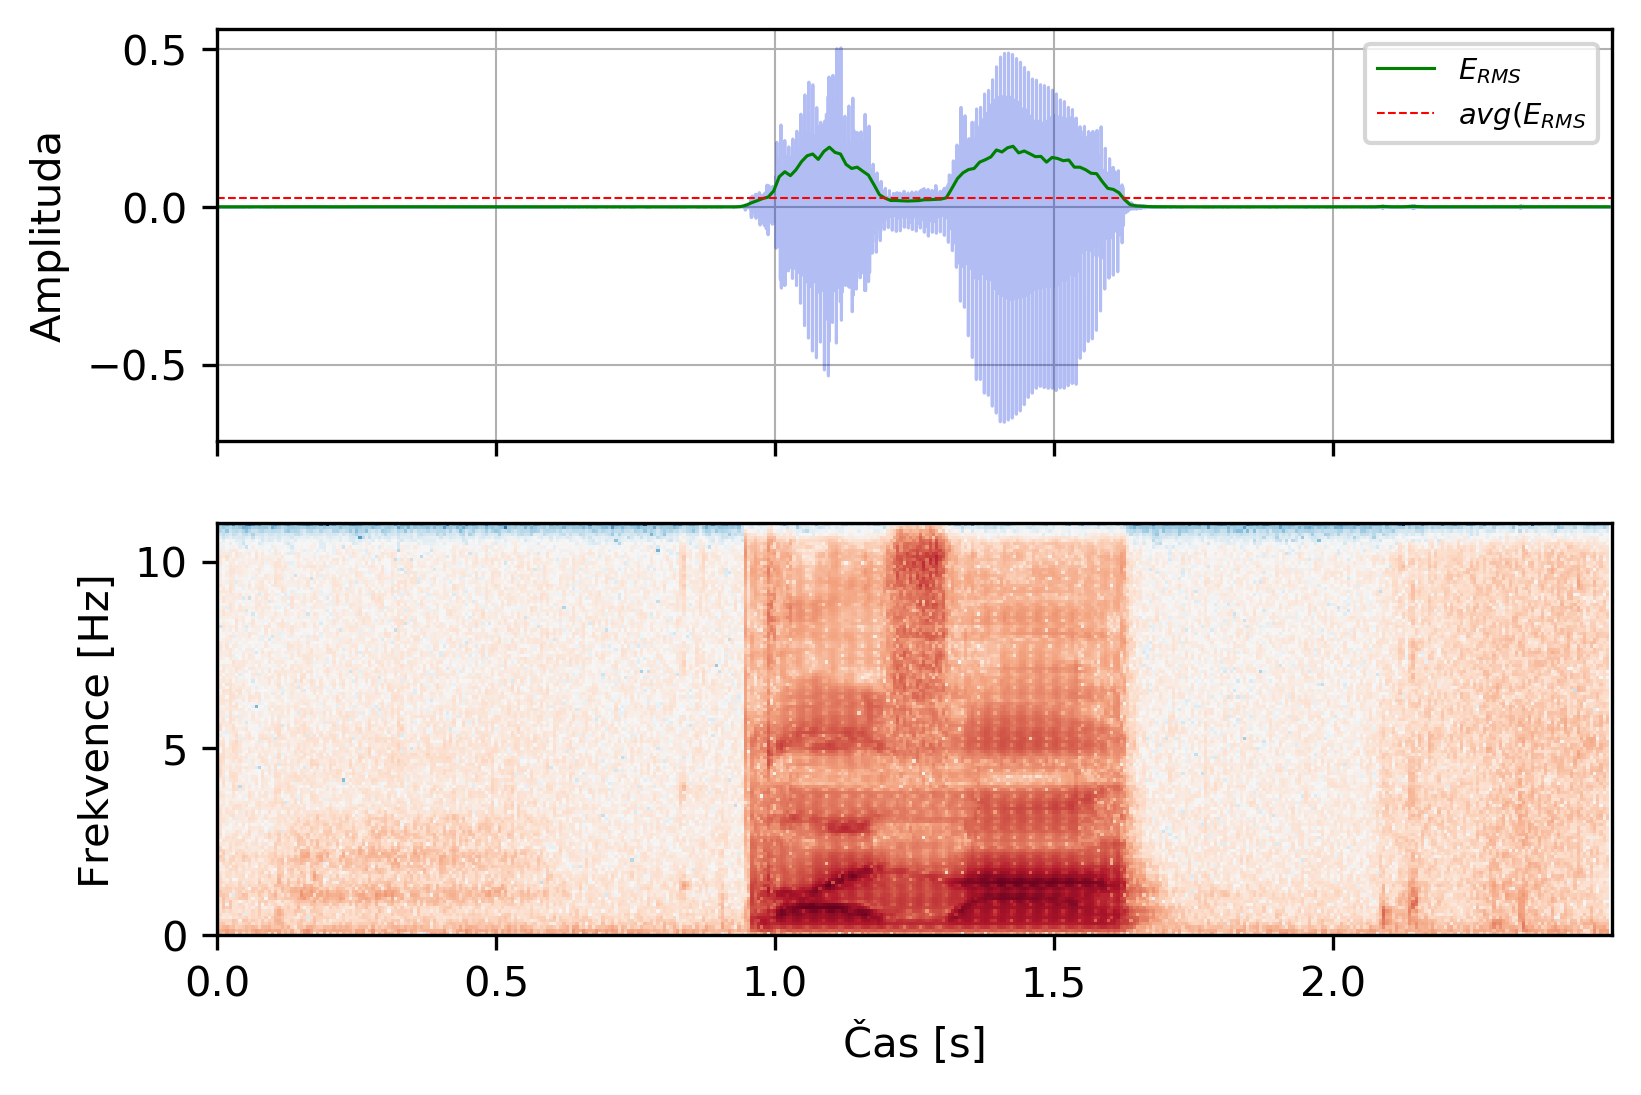
\includegraphics[width=0.9\textwidth]{./ch4-experiments/img/energy_spec_word.png}
  \caption{Průběh a spektrogram slova \uv{kosa} s společně s vyznačenou energií EL promluvy.}
  \label{fig:experiments:normalization:word}
\end{figure}

\begin{figure}[hbpt]
  \centering
  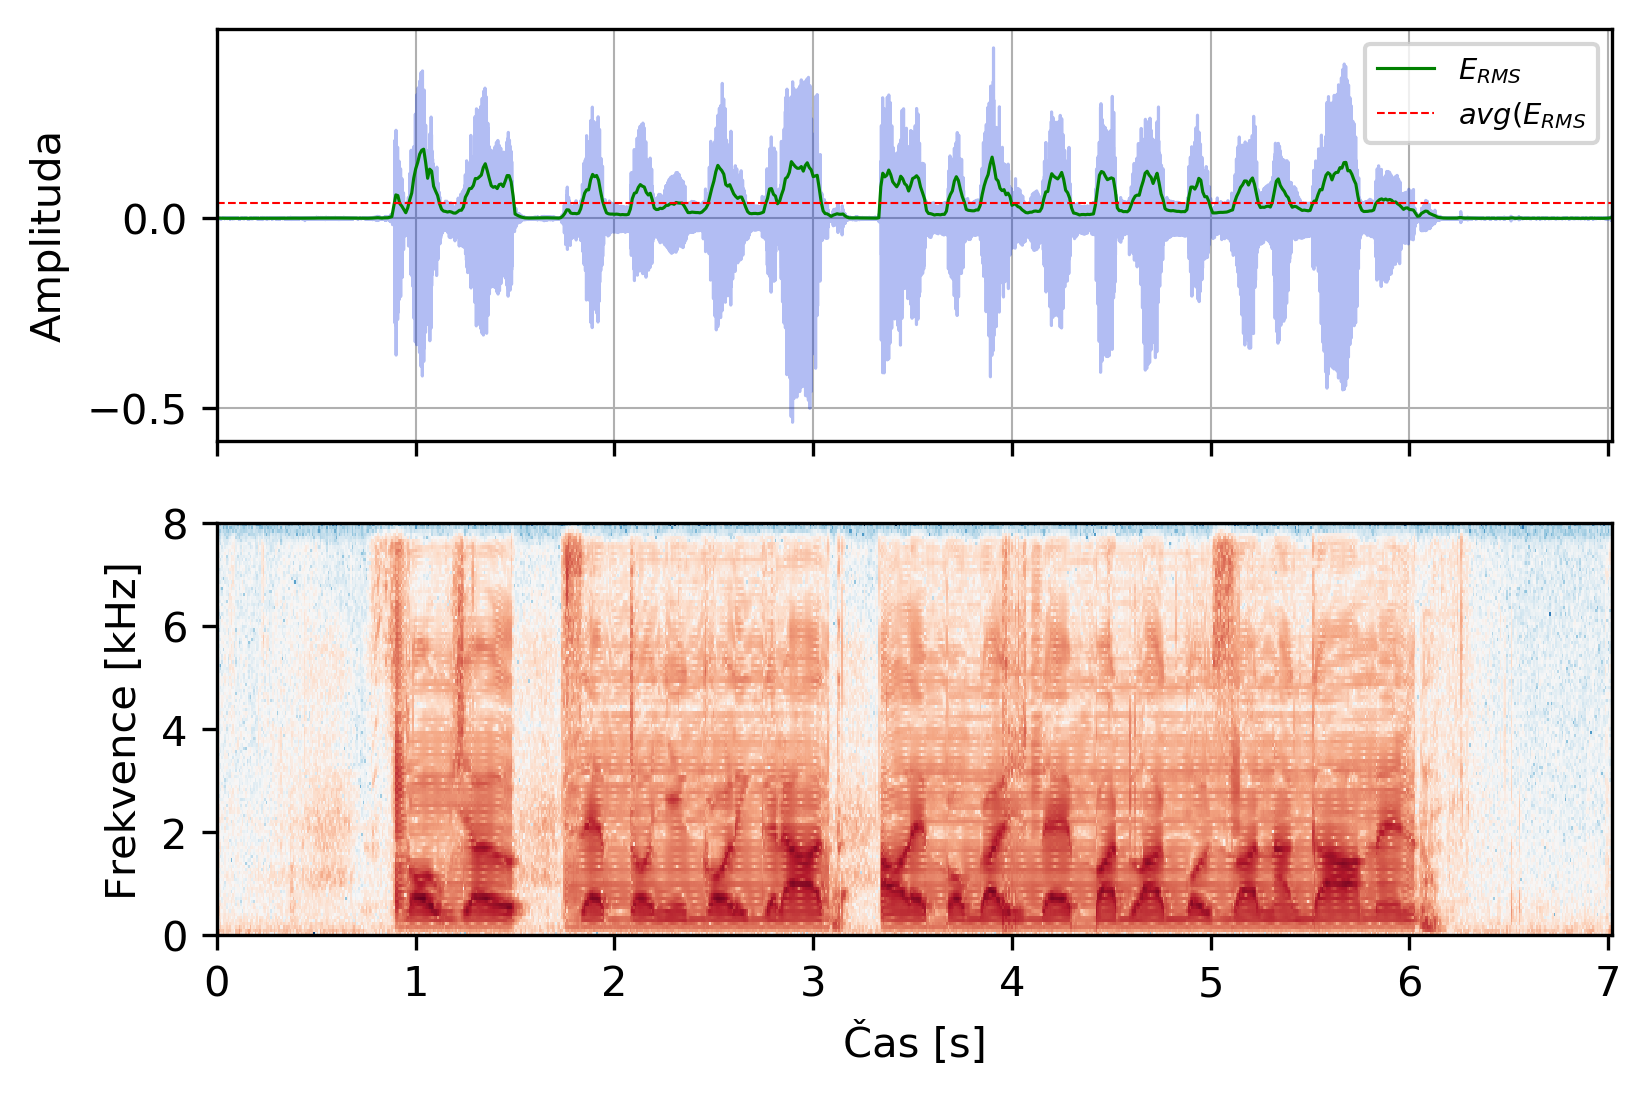
\includegraphics[width=0.9\textwidth]{./ch4-experiments/img/energy_spec_sentence.png}
  \caption{Průběh a spektrogram promluvy obsahující slovo \uv{kosa} a vyznačenou energií EL promluvy.}
  \label{fig:experiments:normalization:sentence}
\end{figure}

Celkem se v 2. etapě pořídila přibližně 1 hodina řečových dat. Celý korpus po 2. etapě tak obsahuje 11 hodin řečových dat, sestávajích z více než $5400$ vět a $320$ izolovaných slov.

\subsection{Vliv nových dat na kvalitě modelů}
\label{chap:experiments:normalization:corpus}

TBD

Z dosažených výsledků vyplývá, že nová data jsou příliš odlišná od původních dat. Zároveň je těchto dat relativně malé množství, aby se mohly modely adaptovat. Na rozdíl v datech se můžeme koukat jako na změnu kanálu, která je příčinou změn v datech, protože řečník je stejný. V předchozím textu bylo zmíněno, že v rámci druhé etapy došlo ke změné nahrávací procedury. Tím byl pozměněn kanál a logicky výsledná zaznamenaná řeč má jiné parametry než ta v 1. etapě. Mezi další prvky, které mohou způsobit změnu kanálu může být prostředí, tedy jestli je řeč produkována uvnitř nějaké místnosti, či venku, jestli je na pozadí přítomen šum atp. K tomu, aby bylo možné použít všechna dostupná data, je potřeba eliminovat vliv kanálu. K jeho eliminaci je možné využít CMN, což je zkratka anglických slov Cepstral Mean Normalisation.

Zaznamenaný signál je možné popsat jako

\begin{equation}
  y\left[n\right] = x\left[n\right] \circledast h\left[n\right],
  \label{eq:experiments:normalization:convolution}
\end{equation}

\noindent kde $x\left[n\right]$ představuje vstupní signál, tedy řeč, a $h\left[n\right]$ odezva kanálu na jednotkový impulz. Zaznamenaný signál je pak jejich lineární konvolucí. Ve frekvenční oblasti pak rovnice \ref{q:experiments:normalization:convolution} zapsaná nýsledovně:

\begin{equation}
  Y\left[f\right] = X\left[f\right] \cdot H\left[f\right]
\end{equation}

\noindent Ve frekvenční oblasti se z konvuluce stalo násobění což značně zjednodušuje situaci. K odstranění vlivu kanálu je, ale ještě potřeba převést hodnoty do kepstrálná oblasti. To je realizováno pomocí logaritmu spektra

\begin{equation}
  Y\left[q\right] = \log\left(Y\left[f\right]\right) = \log\left(X\left[f\right] \cdot H\left[f\right]\right) = X\left[q\right] + H\left[q\right],
\end{equation}

\noindent kde $q$ představuje kepstrální koeficient. V kepstrální oblasti je vliv kanálu aditivní složkou výsledného záznamu. Problémem však je, že konkrétní hodnota vlivu kanálu je neznáma, protože k dispozici je pouze výsledný ovlivněný signál. Předpokládejme však, že vliv kanálu je stacionární\footnote{Jedná se sice o silný, ale logický předpoklad. Pokud se vztáhne k pořízenému řečovému korpusu, tak v rámci jedné etapy nahrávání, je proces nahrávání neměnný, tzn. je použita stejná aparatura a k nahrávání dochází vždy ve stejné místnosti.}, tak poté je možné každý frame nahrávky $i$ zapsat jako

\begin{equation}
  Y_i\left[q\right] = H\left[q\right] + X_i\left[q\right],
\end{equation}

\noindent kde $Y_i\left[q\right]$ představuje $i-\text{tý}$ frame kepstra $q$ nahrávky a $X_i\left[q\right]$ představuje $i-\text{tý}$ frame kepstra $q$ neovlivněné řeči. Z této rovnice je pak možné vypočítat střední hodnotu

\begin{equation}
  \frac{1}{N} \sum_i Y_i\left[q\right] = H\left[q\right] + \frac{1}{N} \sum_i X_i\left[q\right].
\end{equation}

\noindent Vliv kanálu je pak možné eliminovat odečtením střední hodnoty kepstra $q$ od aktuální hodnoty kepstra $Y_i\left[q\right]$

\begin{align}
  R_i\left[q\right] &= Y_i\left[q\right] - \dfrac{1}{N}\sum_{j} Y_j\left[q\right] \nonumber  \\
  &= H\left[q\right] + X_i\left[q\right] - \left( H\left[q\right] + \frac{1}{N} \sum_j X_j\left[q\right] \right) \nonumber  \\
  &= X_i\left[q\right] - \frac{1}{N} \sum_j X_j\left[q\right]
  \label{eq:experiments:normalization:cmn}
\end{align}

\noindent S pomocí rovnice \ref{eq:experiments:normalization:cmn} je možné odfiltrovat vliv kanálu a teoreticky by tak získat hodnoty kepstrálních koeficientů odpovídající nezkreslené řeči.

\subsection{Poslechový test}

\subsection{Výsledky porovnání}

\begin{itemize}
  \item popsat důvody proč potřebujeme další nahrávky (slova, která se liší znělostí)
  \item popsat algoritmus výberu slov/vět k nahrávání
  \item napsat něco o tom, že mezi nahráváními byl velký časový rozestup a taky se změnila technika nahráváními
  \item problém taky s tím, že první sada nahrávek je mnohem větší (10h) než ta nová (cca 30 min) a modely tak nefungovali na nových datech v testovací sade
  \item použití neuronovek (Kaldi)
  \item popis a výsledky experimentu \uv{člověk vs. stroj}
\end{itemize}
